% Official Springer Nature journal class; IEC author guidelines take precedence.
% Results and outstanding tests remain on hold at the authors' request.
\documentclass[pdflatex,sn-mathphys-num,referee,a4paper]{sn-jnl}
\usepackage{graphicx}
\usepackage{booktabs}
\usepackage{amsmath}
\usepackage{xcolor}
\begin{document}
\title{Machine Learning for Cyclone Prediction in the Bay of Bengal}
\author*[1]{\fnm{Md. Faisal} \sur{Tabrez}}\email{faisaltabrez01@gmail.com}
\author[1]{\fnm{K.} \sur{Akhilesh}}\email{akhlieshkancharla05@gmail.com}
\author[1]{\fnm{T. V.} \sur{Rajinikanth}}
\affil[1]{\orgdiv{Department of Computer Science and Engineering}, \orgname{Mahatma Gandhi Institute of Technology}, \orgaddress{\city{Hyderabad}, \state{Telangana}, \country{India}}}
\abstract{This study investigates whether compact machine learning models improve six hour cyclone track and intensity prediction in the Bay of Bengal relative to physical references. A retrospective framework combines historical storm states, atmospheric reanalysis and sea surface temperature while retaining missing inputs and partially observed intensity labels. Residual snapshot, recurrent and tree models are compared using chronological partitions that keep complete storm lifecycles together. Deterministic selection, uncertainty calibration and final testing use separate roles. A Gaussian spread network estimates uncertainty around a fixed ensemble, with comparison against constant spread and uncalibrated forecasts using proper scoring rules. Comparisons preserve identical evaluation populations. The contribution is a reproducible regional comparison protocol that makes labelled populations, forecast references and experiment chronology explicit. Performance results and related conclusions remain on hold pending completion of the study. The framework supports research towards coastal preparedness; operational warning capability and quantified disaster impact have not been established.}
\keywords{Tropical cyclone, Bay of Bengal, Residual learning, Missing data, Predictive uncertainty, Disaster preparedness}
\maketitle
\noindent\textbf{Notation.} $t$: current observation time; NIO: North Indian Ocean; ERA5: ECMWF reanalysis; OISST: optimum interpolation sea surface temperature.

\section{Introduction}
Cyclone position and intensity information can inform coastal preparedness, but a useful regional model must improve on simple references under a defensible evaluation. Closely spaced observations, incomplete intensity records and retrospective environmental products complicate that comparison. The primary question is whether compact residual models improve six-hour predictions for later, unseen Bay-affecting storms. A related question is whether a calibrated uncertainty model improves proper scores relative to declared spread references while keeping point forecasts fixed.

Giffard-Roisin et al. combined trajectories and spatial reanalysis for 24-hour track forecasting \cite{giffard2020}. Mawatwal and Das studied satellite-based intensity estimation in the North Indian Ocean and contrasted chronological independent testing with stratified splitting \cite{mawatwal2024}. Their target is intensity estimation rather than this study's six-hour prediction from current states. Fernandez et al. estimated track-forecast uncertainty with a neural bivariate Gaussian \cite{fernandez2025}. Gaussian track uncertainty is therefore established prior work. Different inputs, populations and lead times preclude direct numerical comparisons with those studies.

This study contributes an integrated regional comparison protocol for track, wind, pressure and predictive uncertainty, with explicit label populations and separate selection, calibration and testing roles. Snapshot and tree controls test whether recurrent history is necessary, consistent with the importance of strong tabular baselines \cite{gorishniy2021}. The study does not assert a new architecture or first regional application.


\section{Data and labelled populations}
At an existing cyclone observation time t, the targets are position, maximum sustained wind and minimum central pressure six hours later. The derived 1982-2025 package combines the International Best Track Archive for Climate Stewardship, IBTrACS v04r01 \cite{knapp2010,gahtan2024}, Optimum Interpolation Sea Surface Temperature, OISST v2.1 \cite{huang2021}, and European Centre for Medium-Range Weather Forecasts (ECMWF) ERA5 atmospheric reanalysis \cite{hersbach2020}. Main tracks are filtered to synoptic hours and continuous six-hour pairs. New Delhi intensity fields are preferred, with World Meteorological Organization (WMO) values as fallback.

Table 1 gives whole-storm roles. The broader North Indian Ocean (NIO) training set includes every Bay training row and adds 997 pairs from 54 storms; it is not an independent additional sample. Bay-affecting lifecycles include positions outside the geographic Bay box, defined here as 5-25 degrees north and 78-100 degrees east. Selection and calibration divide validation by complete storm; boundary-spanning storms enter the later role. The full validation archive was inspected during earlier baseline acceptance, so calibration is reserved from learned-model selection rather than described as never inspected.

Only 2334 of 4560 Bay training pairs have wind targets and 2267 have pressure targets, approximately 51.2\% and 49.7\%. Some observed future labels lack a current measurement. Supplement S1 reports observed-target and persistence-eligible counts by accessible partition. Masking preserves usable observations but does not establish that the labelled intensity population represents all storms. Changing reporting coverage over time limits generalisation.

The 39 predictors cover storm state, tendencies, calendar, location and centre-linked environmental quantities. SST outside the supplied regional crop remains missing with an availability flag. Supplement S1 specifies the ordered features, units, transformations and unresolved acquisition details. Reproducibility is currently from the supplied derived package; original extraction notebooks are needed for complete raw-source reproduction.


\begin{table}[htbp]
\caption{Dataset roles and observed wind/pressure target counts. NIO includes Bay training. Final-test pair/storm counts are metadata; label auditing remains on hold. Persistence-eligible counts are in Supplement S1.}\label{tab:data}
\centering
\begin{tabular}{p{43mm}rrr}
\toprule
Role and years & Pairs / storms & Wind & Pressure \\
\midrule
Bay training (1982-2010) & 4560 / 235 & 2334 & 2267 \\
NIO incl. Bay (1982-2010) & 5557 / 289 & 2848 & 2742 \\
Selection (2011-2014) & 493 / 25 & 349 & 347 \\
Calibration (2015-2017) & 361 / 25 & 298 & 303 \\
Test metadata (2018-2025) & 1018 / 65 & held & held \\
\bottomrule
\end{tabular}
\end{table}

\section{Residual models and selection}
Each feature is standardised using training statistics and paired with a missingness indicator, producing 78 inputs. Missing standardised values are zero; near-constant features use unit scale. Missing future labels are excluded before loss arithmetic, while observed targets are retained when current intensity is unavailable.

The track anchor extrapolates the previous six-hour latitude and longitude changes, with persistence fallback. Anchor and target positions are represented in the tangent plane at the current centre using a spherical logarithmic map. Intensity anchors use current observations or training current-feature means. For the transformed target vector y, anchor a and diagonal training scale matrix S, the model learns the scaled residual and reconstructs the forecast as follows.

\begin{equation}
\mathbf{r}_t=S^{-1}(\mathbf{y}_{t+6}-\mathbf{a}_t),\qquad \widehat{\mathbf{y}}_{t+6}=\mathbf{a}_t+S f_{\theta}(\mathbf{x}_{\leq t})
\end{equation}
A common track scale is the training root-mean-square magnitude across the two residual coordinates; wind and pressure have separate scales, each bounded below by one native unit. Corrected track displacement is decoded by the spherical exponential map. Zero output reproduces the anchor. The snapshot multilayer perceptron (MLP) uses widths 78, 64, 32 and 4. The gated recurrent unit (GRU) projects inputs to 32 features, uses hidden width 64 and concatenates its final state with current projected features before three task heads. Up to four consecutive observations span 18 hours; short initial sequences are retained. Snapshot inputs already contain engineered six-hour tendencies.

Candidates are Bay-only MLP, GRU and boosted trees; NIO-pretrained GRU with Bay fine-tuning; and pooled NIO GRU without fine-tuning. The original objective equally weights active track, wind and pressure tasks using masked SmoothL1 residual losses. A bounded, post-inspection development follow-up compares the original MLP, persistence replacement for observed current wind, and absolute wind loss with other losses unchanged. This is exploratory development, not independent confirmation.

Candidate families use seeds 17, 29 and 43. A seed's checkpoint minimises the composite score J below; family selection uses the mean individual-seed score. The final point predictor averages the selected family's three forecasts in common tangent-plane and native intensity coordinates. T and Tcv denote mean track errors; W and P denote paired intensity mean absolute errors, with Wpers and Ppers their persistence references.

\begin{equation}
J=\frac{1}{3}\left(\frac{T}{T_{\mathrm{cv}}}+\frac{W}{W_{\mathrm{pers}}}+\frac{P}{P_{\mathrm{pers}}}\right)
\end{equation}
Intensity ratios use identical rows with observed current and future intensity. All-observed-label errors are reported separately. Supplement S1 records optimiser schedules, model heads, tree settings and transfer normalisation rebasing. Any causal transfer-benefit claim requires controls for optimisation budget and repeated Bay exposure.


\section{Uncertainty and reference forecasts}
Point-model weights remain fixed during uncertainty learning. A separate 78-32-5 MLP predicts four positive standard deviations and track correlation, defining one Gaussian around the ensemble rather than a member mixture. Track is bivariate; wind and pressure are independent marginals. This omits cross-task dependence. Softplus scales have native floors equivalent to 1 km per track axis, 0.2572 metres per second (0.5 knots) and 50 Pa (0.5 hPa). Correlation is bounded by 0.95 times a hyperbolic tangent.

Spread learning minimises scale-normalised Gaussian negative log likelihood with equal active-task weights and selection-based checkpoint choice. In-sample training error RMS initialises spread and is not an out-of-fold uncertainty estimate. After the mean and spread model is frozen, three factors in [0.25, 4] scale track, wind and pressure on reserved calibration storms. Track covariance changes by the factor squared; means and correlation remain fixed. Calibration-fit diagnostics are not independent validation.

All probability forecasts share the same frozen means. Declared references are a constant diagonal Gaussian using the frozen training-error RMS scales and zero track correlation, and the uncalibrated learned Gaussian. The candidate is the calibrated learned Gaussian. Paired proper-score differences assess the complete workflow; these comparisons do not isolate every contribution of input-dependent spread, correlation or calibration. Figure 1 summarises the workflow.


\begin{figure}[htbp]
\centering
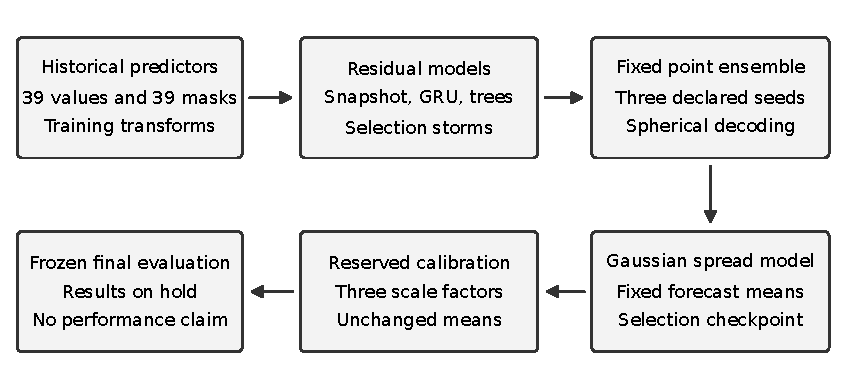
\includegraphics[width=\linewidth]{figures/workflow.pdf}
\caption{Residual prediction and frozen-mean uncertainty workflow. Reserved calibration adjusts spread; the final-test stage remains on hold.}\label{fig:workflow}
\end{figure}

\section{Evaluation and reproducibility}
Point reporting includes great-circle track mean, median and 90th percentile, intensity mean absolute errors, persistence/constant-velocity references and storm-macro summaries. Probability reporting includes native-unit negative log likelihood, marginal continuous ranked probability score, spatial energy score using 512 fixed-seed draws, and 50\%, 80\% and 90\% coverage with interval width or ellipse area. Proper scores complement coverage \cite{gneiting2007}. Track densities are defined in tangent-plane kilometres, not latitude-longitude or spherical-area density.

Descriptive 95\% percentile intervals use 2000 whole-cyclone bootstrap replicates. Paired model-reference differences use the same storms and eligible rows. Complete lifecycles and the geographic Bay subset are reported separately with storm and label counts. Reused selection data, calibration-fit diagnostics and final-test findings have distinct interpretations. No adaptation to final-test outcomes is permitted.

Supplement S1 binds the dataset, feature order, role assignments, current method-source files and configuration snapshots with checksums. It separates current documentation from historical training-source receipts. Acceptance checks establish execution rather than predictive skill. Exact source-download times, interpolation choices and daily SST temporal support remain unresolved and are identified explicitly.


\section{Results on hold}
Model comparisons, required outstanding tests and final-test findings remain on hold. The completed results account will distinguish original development, the later wind-loss follow-up, calibration-fit diagnostics and frozen final evaluation. Performance statements in the abstract and conclusion will depend on those verified findings.


\section{Discussion and limitations}
The experiment is retrospective. Best-track revision, reanalysis release latency and the support of daily SST prevent assuming real-time availability from causal row ordering. Same-date SST can include observations acquired after an early forecast origin. Operational use requires a source-timing audit and latency-matched predictors and references.

Incomplete labels, reporting conventions, structured SST missingness and temporal/geographic shifts can affect generalisation. Observed-target counts do not reveal the intensities of unreported targets. Gaussian wind permits negative mass and pressure is unbounded; diagnostics report that mass without clipping. Row-weighted calibration and few calibration storms do not imply population-wide coverage guarantees.

The intended application is research towards coastal preparedness and infrastructure resilience. Energy savings, avoided losses and operational decision benefits require separate measurements. The protocol tests forecast skill; it does not estimate cyclone genesis, inundation or administrative-state landfall.


\section{Conclusion}
The study specifies a regional comparison of compact residual models and frozen-mean uncertainty estimation under chronological storm-level evaluation. Explicit label populations and matched references define what the eventual evidence can support. Comparative performance conclusions remain on hold.


\backmatter

\subsection*{Acknowledgements}
NOAA NCEI and ECMWF/Copernicus provide the underlying data. Contains modified Copernicus Climate Change Service information 2026. The providers do not endorse the study.

\subsection*{Funding}
Author confirmation pending.

\subsection*{Competing interests}
Author confirmation pending.

\subsection*{Author contributions}
Individual contributions and final author approval are pending confirmation.

\subsection*{Data and code availability}
The project repository is https://github.com/FaisalTabrez/bay-of-bengal-cyclone-ai. Supplement S1 v1 documents the derived-package contract, accessible label counts and method/configuration snapshots. Provider terms apply separately. Code licensing, original extraction notebooks and the final results archive remain unresolved.

\subsection*{AI assistance}
OpenAI Codex assisted with literature lookup, drafting and formatting. The authors retain responsibility for verification and the final text.

\begin{thebibliography}{9}
\interlinepenalty=10000
\bibitem{giffard2020}
Giffard-Roisin S, Yang M, Charpiat G, Kumler Bonfanti C, Kegl B, Monteleoni C (2020) Tropical Cyclone Track Forecasting Using Fused Deep Learning From Aligned Reanalysis Data. Frontiers in Big Data 3:1. \url{https://doi.org/10.3389/fdata.2020.00001}

\bibitem{mawatwal2024}
Mawatwal MK, Das S (2024) An End-to-End Deep Learning Framework for Cyclone Intensity Estimation in North Indian Ocean Region Using Satellite Imagery. Journal of the Indian Society of Remote Sensing 52:2165-2175. \url{https://doi.org/10.1007/s12524-024-01929-8}

\bibitem{fernandez2025}
Fernandez MA, Barnes EA, Barnes RJ, DeMaria M, McGraw M, Chirokova G, Lu L (2025) Predicting Tropical Cyclone Track Forecast Errors Using a Probabilistic Neural Network. Artificial Intelligence for the Earth Systems 4:e240066. \url{https://doi.org/10.1175/AIES-D-24-0066.1}

\bibitem{gorishniy2021}
Gorishniy Y, Rubachev I, Khrulkov V, Babenko A (2021) Revisiting Deep Learning Models for Tabular Data. Advances in Neural Information Processing Systems 34:18932-18943. \url{https://proceedings.neurips.cc/paper/2021/hash/9d86d83f925f2149e9edb0ac3b49229c-Abstract.html}

\bibitem{knapp2010}
Knapp KR, Kruk MC, Levinson DH, Diamond HJ, Neumann CJ (2010) The International Best Track Archive for Climate Stewardship (IBTrACS): Unifying tropical cyclone best track data. Bulletin of the American Meteorological Society 91:363-376. \url{https://doi.org/10.1175/2009BAMS2755.1}

\bibitem{gahtan2024}
Gahtan J, Knapp KR, Schreck CJ, Diamond HJ, Kossin JP, Kruk MC (2024) International Best Track Archive for Climate Stewardship (IBTrACS) Project, Version 4r01. North Indian Ocean subset. NOAA National Centers for Environmental Information. \url{https://doi.org/10.25921/82ty-9e16}

\bibitem{huang2021}
Huang B et al. (2021) Improvements of the Daily Optimum Interpolation Sea Surface Temperature (DOISST) Version 2.1. Journal of Climate 34:2923-2939. \url{https://doi.org/10.1175/JCLI-D-20-0166.1}

\bibitem{hersbach2020}
Hersbach H et al. (2020) The ERA5 global reanalysis. Quarterly Journal of the Royal Meteorological Society 146:1999-2049. \url{https://doi.org/10.1002/qj.3803}

\bibitem{gneiting2007}
Gneiting T, Raftery AE (2007) Strictly proper scoring rules, prediction, and estimation. Journal of the American Statistical Association 102:359-378. \url{https://doi.org/10.1198/016214506000001437}

\end{thebibliography}
\section*{List of captions}
Table 1. Dataset roles and observed wind/pressure target counts. NIO includes Bay training. Final-test pair/storm counts are metadata; label auditing remains on hold. Persistence-eligible counts are in Supplement S1.

Figure 1. Residual prediction and frozen-mean uncertainty workflow. Reserved calibration adjusts spread; the final-test stage remains on hold.
\end{document}
